\vspace*{\fill}
\begin{center}
    {\color{Black} \rule{\linewidth}{1.2mm} }\\
\vspace{0.25in}
{\centering\fontsize{30}{40}{\bfseries{\color{Black}{\scshape{Chapter I : Blood cells \& artificial intelligence}}}}}
\vspace{0.35in}\\
    {\color{Black} \rule{\linewidth}{1.2mm} }
\end{center}
\vspace*{\fill}
\addcontentsline{toc}{chapter}{\color{Black}{Chapter I : Blood cells \& artificial intelligence}}
\setcounter{section}{0}

\newpage

\section{Introduction}
\vspace{0.2in}
\hspace{\parindent}
In this chapter, we will present to you the blood cells and it's three main types (red, white blood cells and platelets) as well as the complete blood count and the purpose of it. Then, we will present some of the many diseases related to blood cells, and how can we detect and avoid them using artificial intelligence techniques.

\section{Blood cell}
\subsection{Definition}
\hspace{\parindent}
A blood cell, also called a hematopoietic cell, hemocyte, or hematocyte, is a cell produced through hematopoiesis and found mainly in the blood. Major types of blood cells include red blood cells (erythrocytes), white blood cells (leukocytes), and platelets (thrombocytes). Together, these three kinds of blood cells (as we can see in fig\ref{fig:bloodCellTypes}) add up to a total 45\% of the blood tissue by volume, with the remaining 55\% of the volume composed of plasma, the liquid component of blood. \textsuperscript{\cite{hopkins1993human}}\\

\begin{figure}[h]
\centering
  \vspace{-0.2in}
    \centerline{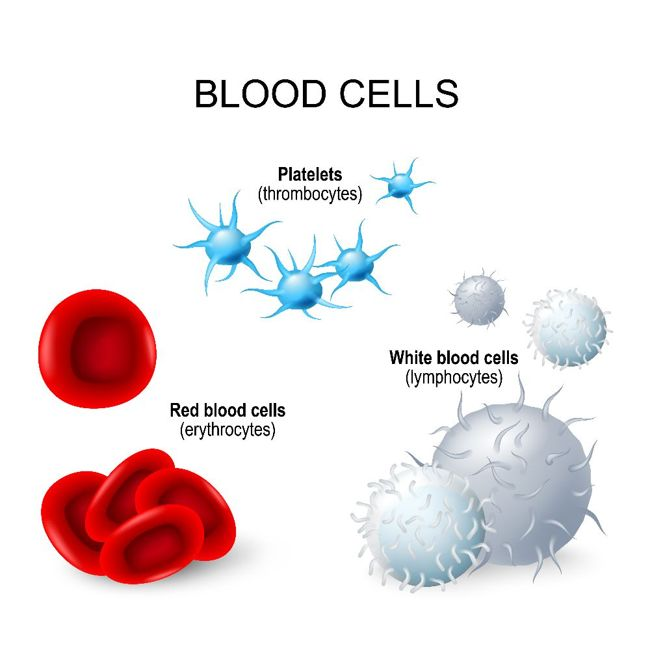
\includegraphics[width = 2.2in]{../images/BloodCells.jpg}}
    \caption{Blood Cell Types}
    \label{fig:bloodCellTypes}
\end{figure}

That said, there are three main types of blood cells:

\subsection{Red blood cells}
\hspace{\parindent}
Red blood cells (RBCs) are the cells which carry fresh oxygen all over the human body. This is vital to our health. They are round with a flattish, indented center, like doughnuts without a hole. 
The hemoglobin is the protein found inside the red blood cell, and it's main purpose is carrying oxygen.\

Most people don't think about their red blood cells unless they have a disease that affects these cells. Problems with red blood cells can be caused by illnesses or a lack of iron or vitamins. Some diseases of the red blood cells are inherited.

Diseases of the red blood cells include many types of anemia. This is a condition in which there are too few red blood cells to carry enough oxygen all over the body.

People with anemia may have red blood cells that have an abnormal shape or that look normal, larger than normal, or smaller than normal.

Symptoms of anemia include tiredness, fast heart rate, pale skin, feeling cold, and, in severe cases, heart failure. Children who don't have enough healthy red blood cells grow and develop more slowly than other children. These symptoms show how important red blood cells are to your daily life. \textsuperscript{\cite{RBC-urmcrochester}}

\subsection{White blood cells}
\hspace{\parindent}
On the other hand, White blood cells (WBCs), also known as leukocytes, are the ones responsible for protecting the human body from infections. As part of the immune system, These cells circulate in the blood and respond to injury or illness. They travel through the bloodstream searching for infections. Then, they notify other WBCs of their location to help defending against attacks from other unknown organisms. Once the army of WBCs arrive, they fight the invader by producing antibody proteins to attach to the organism and destroy it. \textsuperscript{\cite{WBC-clevelandclinic}}

White blood cells are divided into five types:

\begin{itemize}
  \item \textbf{Neutrophils:} Help protect your body from infections by killing bacteria, fungi and foreign debris.
  \vspace{-0.05in}
  \item \textbf{Lymphocytes:} Consist of T cells, natural killer cells and B cells to protect against viral infections and produce proteins to help you fight infection (antibodies).
  \vspace{-0.05in}
  \item \textbf{Eosinophils:} Identify and destroy parasites, cancer cells and assists basophils with your allergic response.
  \vspace{-0.05in}
  \item \textbf{Basophils:} Produces an allergic response like coughing, sneezing or a runny nose.
  \vspace{-0.05in}
  \item \textbf{Monocytes:} Defend against infection by cleaning up damaged cells.
\end{itemize}

\begin{figure}[H]
\centering
  \vspace{-0.1in}
    \centerline{\fbox{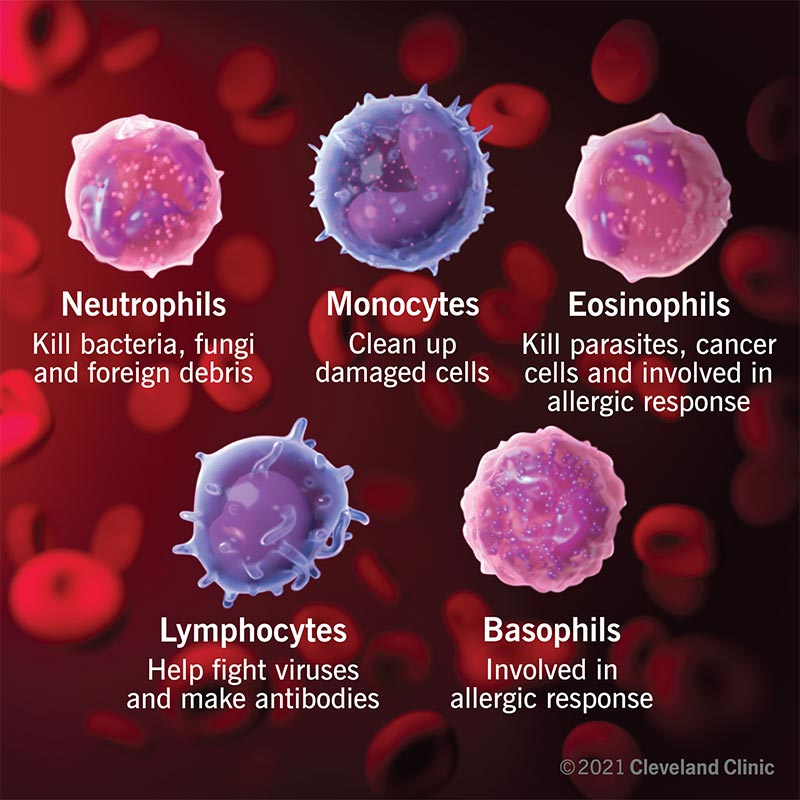
\includegraphics[width = 2.2in]{../images/white_blood_cells.jpg}}}
    \caption{The five types of White blood cells}
\end{figure}

\subsection{Platelets}
\hspace{\parindent}
Platelets help prevent blood loss at sites of vascular injury. To do this, they adhere, aggregate and form a procoagulant surface favorizing thrombin generation and fibrin formation. In addition, platelets express and release substances that promote tissue repair and influence processes such as angiogenesis, inflammation and the immune response. They contain large secretable pools of biologically active proteins, while newly synthesized active metabolites are also released. \textsuperscript{\cite{nurden2008platelets}}

\vspace{0.2in}

\begin{figure}[h]
\centering
  \vspace{-0.1in}
    \centerline{\fbox{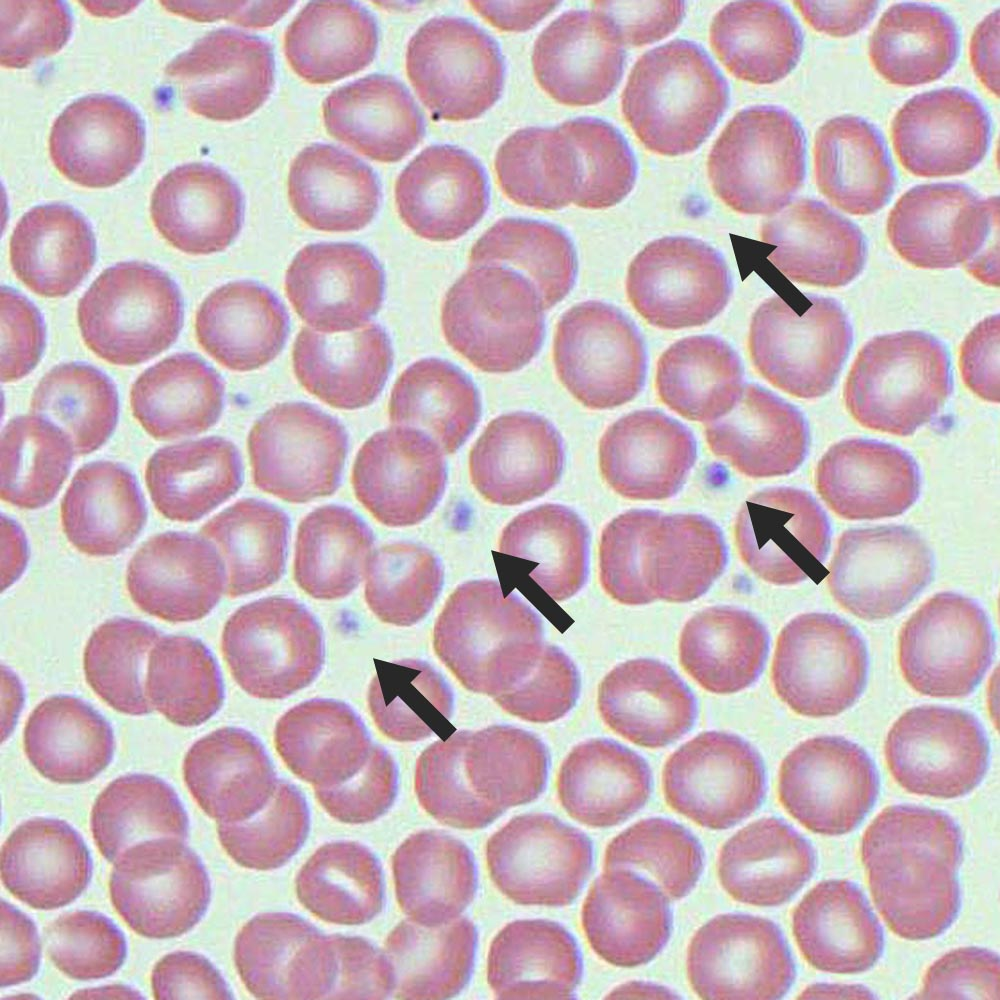
\includegraphics[width = 2.5in]{../images/platelets.jpg}}}
    \caption{Platelets}
\end{figure}

\vspace{-0.1in}

\section{Complete blood count}
\subsection{Definition}
\hspace{\parindent}
A complete blood count (CBC) is a set of tests that gives information about the cells in a person's blood. A scientist or lab technician performs the requested testing and provides the requesting medical professional with the results of the CBC. In the past, counting the cells in a patient's blood was performed manually, by viewing a slide prepared with a sample of the patient's blood under a microscope. Today, this process is generally automated by use of an automated analyzer, with only approximately 10-20\% of samples now being examined manually. Abnormally high or low counts may indicate the presence of a disease.

\subsection{Purpose of a complete blood count}
\hspace{\parindent}
A complete blood count is a common blood test that is done for a variety of reasons:

\begin{itemize}
  \item \textbf{To review the overall health:} A doctor may recommend a complete blood count as part of a routine medical examination to monitor your general health and to screen for a variety of disorders, such as anemia or leukemia.
  \item \textbf{To diagnose a medical condition:} A doctor may suggest a complete blood count if you're experiencing weakness, fatigue, fever, inflammation, bruising or bleeding. A complete blood count may help diagnose the cause of these signs and symptoms. If a doctor suspects someone with an infection, the CBC test can help confirm that diagnosis.
  \item \textbf{To monitor a medical condition:} If you've been diagnosed with a blood disorder that affects blood cell counts, the doctor may use complete blood counts to monitor your condition.
  \item \textbf{To monitor medical treatment:} A complete blood count may be used to monitor your health if you're taking medications that may affect blood cell counts. \textsuperscript{\cite{CBC-mayoclinic}}
\end{itemize}

\subsection{Diseases identified by a complete blood count}
\hspace{\parindent}
Abnormal test results could be an indication of a serious health problem or a simple one that can be remedied by eating better or taking supplements.\\
These are some of the health problems that can be identified by a CBC:

\begin{itemize}
  \item Anemia
  \vspace{-0.05in}
  \item Autoimmune disorders
  \vspace{-0.05in}
  \item Bone marrow problems
  \vspace{-0.05in}
  \item Leukemia (Cancer)
  \vspace{-0.05in}
  \item Dehydration
  \vspace{-0.05in}
  \item Heart disease
  \vspace{-0.05in}
  \item Infection
  \vspace{-0.05in}
  \item Inflammation
  \vspace{-0.05in}
  \item Vitamin and mineral deficiencies
  \vspace{-0.05in}
\end{itemize}

\section{Conclusion}
\hspace{\parindent}
We conclude that there are many diseases related to blood cells, and we must aid in detecting some of them before it is too late.
